% -*- TeX-master: "../fat_manual.tex" -*-

\section{System and amplifiers}
The connections from the top of the system are as follows
\begin{center}
  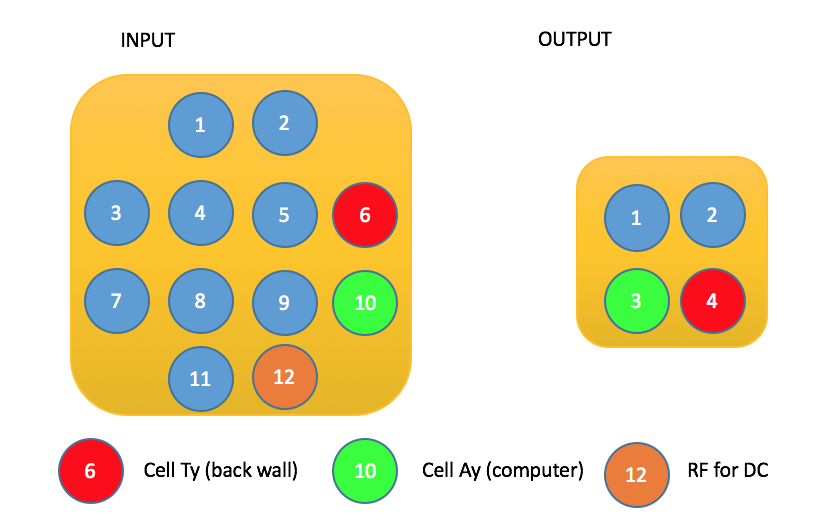
\includegraphics[height=5cm]{top}
  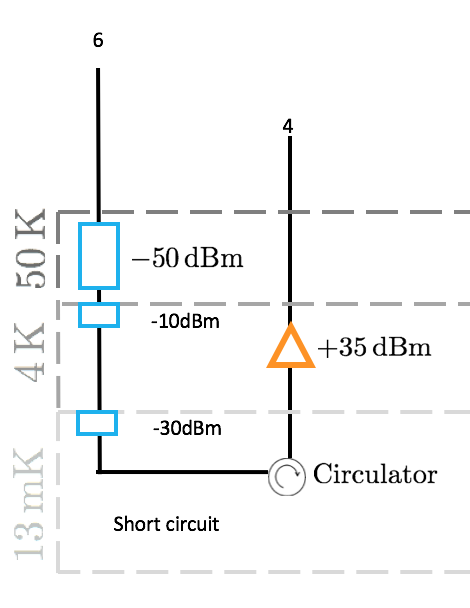
\includegraphics[height=5cm]{side}
\end{center}

\noindent The attenuator markings, which  are attached to the various
plate,   have    the   last   number   depicting    the   atuniation.
\red{\textbf{Note, that it can be 0dB!!!}}
\begin{center}
  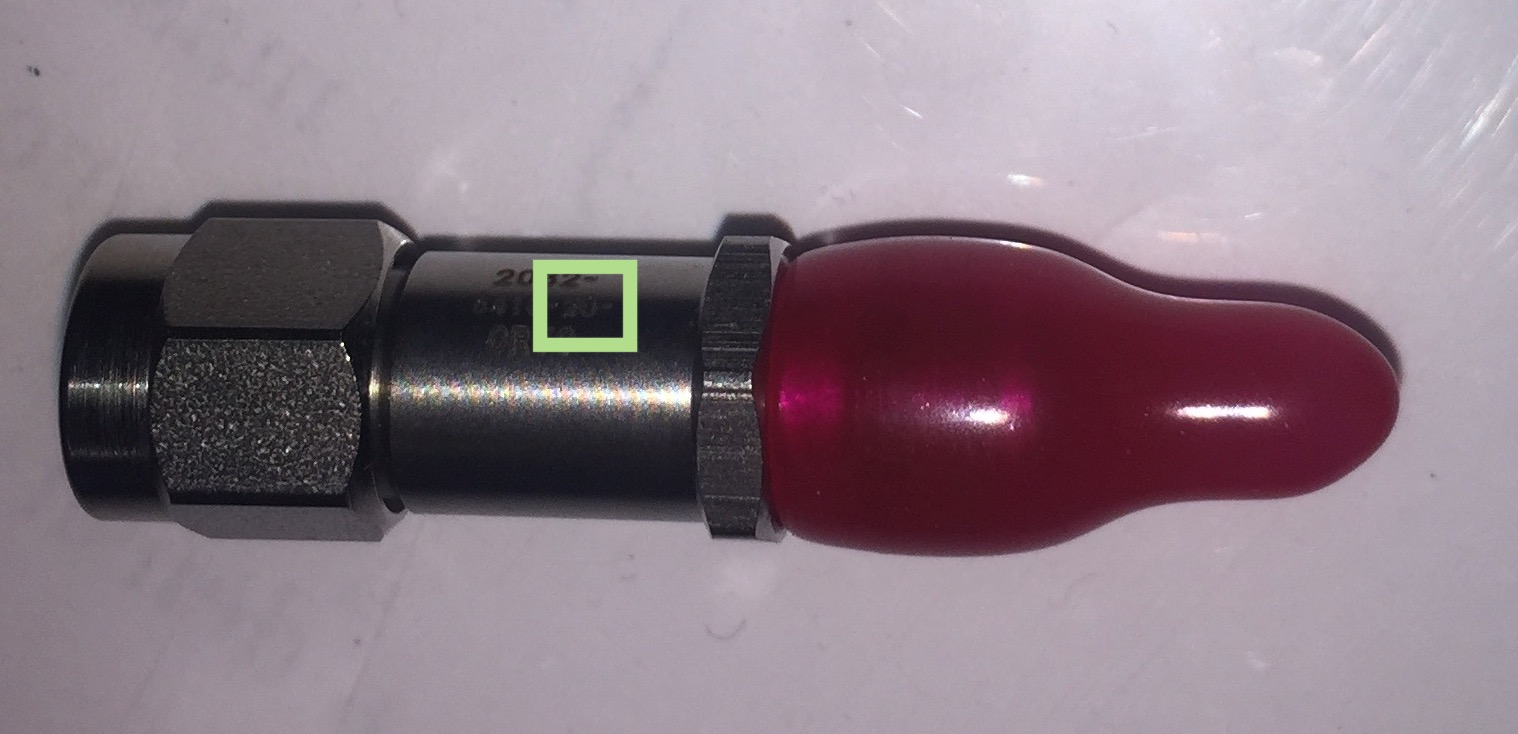
\includegraphics[height=5cm]{filter}
\end{center}

\begin{framed}\noindent
  \red{\textbf{\Large Turn amplifiers off when handling them!}}
\end{framed}

In order to turn  both the room temp and cold  amplifiers on, we need
to apply voltages
\begin{enumerate}
\item
  \href{http://www.lownoisefactory.com/products/roomtemp/1-15-ghz/}{\textbf{LNF-LNR1\_15A}}
  Climb up on the ladder \ira turn  the power supply on \ira turn the
  small  \quote{on}  buttons  at  the bottom  of  the  amplifier  to
  \quote{on} at the same time;
  \[
    \text{Left display:} 2.44V \quad \text{Right display:}2.67\,\text{V}
  \]
\item There are two {LNF-LNR1\_15A} amplifiers:
  \begin{itemize}
  \item Input 10, Output 3, Cell Ay, 337\,V, closer to computer;
  \item Input 6, Output 4, Cell Ty, 330V, closer to back wall;
  \end{itemize}
  On each line there  is a 50dB attenuator in the  top hood, 10dBm on
  the 4K plate  (first grey plate), 30dB on the  13mK plate.  Turn on
  the correct switch on the grey box;
\item                                                              My
  \href{http://www.atlantecrf.com/products/active_components/amplifiers/wide_band_amplifiers.htm}{AOX-010120 amplifier}
  just needs 5\,V from any supply.
\end{enumerate}

\subsubsection{New LNF-LNC4-8C amplifier}
\label{sec:new-lnf-lnc4}


\begin{figure}[h]
  \centering
  \includegraphics[width=1.0\linewidth]{images_inkscape/wiring-lnf-lnc4-8c.pdf}
  \caption{\small Wiring of the amplifier. \label{fig:wiring-lnf-lnc4-8c}}
\end{figure}

The wiring for the newest \texttt{LNF-LNC4\_8C} amplifier is shown in Figure~\ref{fig:wiring-lnf-lnc4-8c}. The small black box (\texttt{LNF-PS3b}) is used to set drain voltage ($V_{d}$) and the drain current ($I_{d}$) through front panel - the gate voltage ($V_{g}$) automatically adjusts.

\textbf{Setup}:
\begin{enumerate}
\item Keep display off for low noise.
\item Switch on the power box \texttt{LNF-PBA}. Install jumper plug between earth and common for non-floating mode;
\item Switch on the black box \texttt{LNF-PS3b} - \textbf{do not connect amplifier yet!};
\item Set $V_{d}=0.7\,\text{V}$;
\item Connect \texttt{LNF-LNC4-8C};
\item Set $I_{d}=15\,\text{mA}$;
\item Can press $V_{d-\text{sense}}$ to show the actual $V_{d}$ on the amplifier. Can correct further;
  \item Can test at room temperature to get 20-30\,dB amplification.
\end{enumerate}

\textbf{Power Off:}
\begin{enumerate}
\item Switch off voltage box \texttt{LNF-PS3b};
\item Switch off the power supply \texttt{LNF-PBA};
\end{enumerate}

\textbf{Power on:}
\begin{enumerate}
\item Switch on power supply \texttt{LNF-PBA};
\item Switch of voltage box \texttt{LNF-PS3b};
\end{enumerate}

\newpage
